\section{Problem 1}

\subsection{Introduction}

This report presents an analysis of the HT R Phase Current dataset. The primary goal is to identify an unstable period within the data and apply various outlier handling techniques, including imputation, trimming, capping, and robust estimation. The findings are illustrated with visualizations, and a statistical comparison of the methods is provided.

\begin{figure}[H]
	\centering
	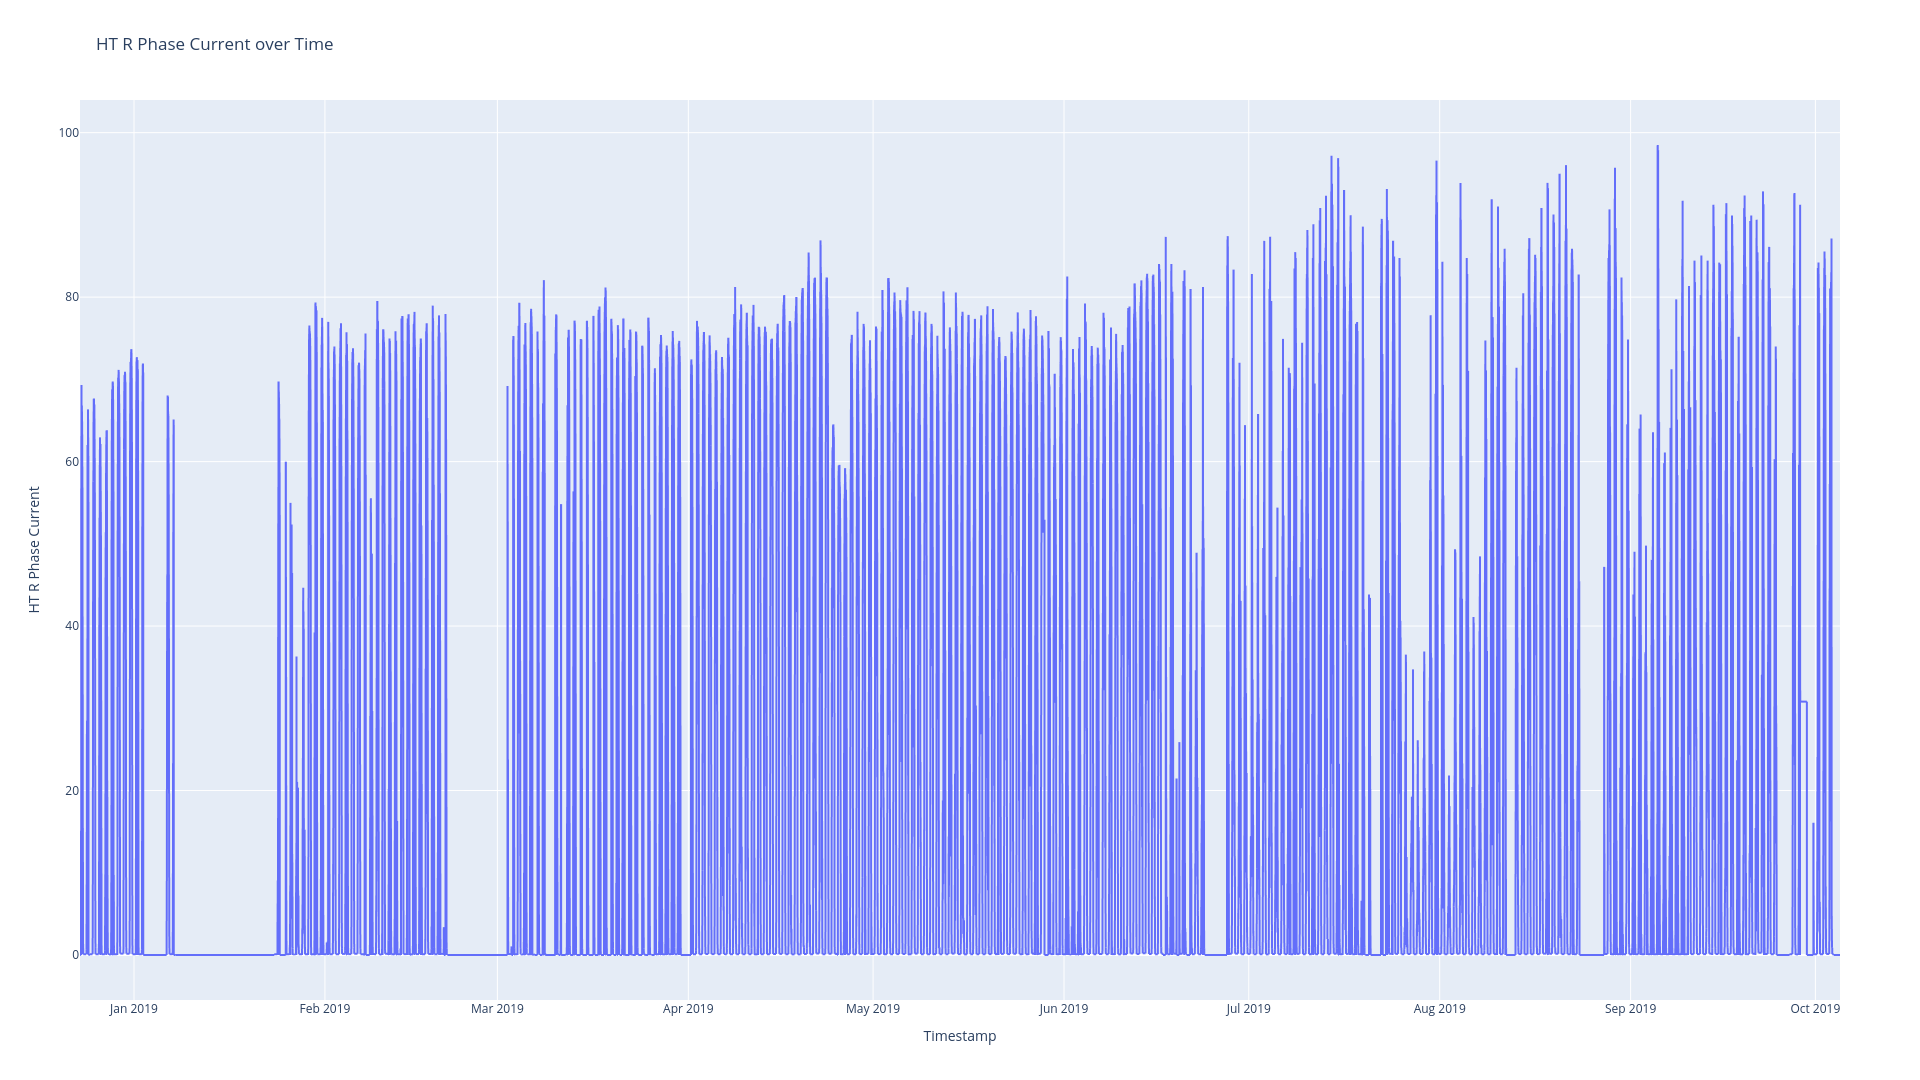
\includegraphics[width=\textwidth]{./Images/ht_r_phase_current.png}
	\caption{HT R Phase Current Dataset}
\end{figure}

\clearpage

\subsection{Data Exploration}

The dataset contains 1,000 records with a mean current of $16.912767$, a standard deviation of $27.174448$, and a range from $0$ to $98.500000$. The data is collected over a period of $9$ Months, with a frequency of $1$ record every $5$ minutes.

% \vspace{2em}

\begin{lstlisting}[language=Python]
import pandas as pd
import numpy as np
import plotly.express as px
import matplotlib.pyplot as plt
from scipy import stats
import os

# Create directory for saving images
if not os.path.exists('Images'):
    os.makedirs('Images')

# Load data from CSV
data = pd.read_csv("e6-htr-current.csv", parse_dates=['Timestamp'], dayfirst=True)

# Part A: Perform EDA
print(data.describe())

# Plot the current over time using Plotly
fig = px.line(data, x='Timestamp', y='HT R Phase Current', title='HT R Phase Current over Time')
fig.write_image("Images/ht_r_phase_current.png", scale=1, width=1920, height=1080, format='png')
fig.show()

# Part B: Identify a 2-week unstable period
unstable_period = data[(data['Timestamp'] >= '2019-07-30') & (data['Timestamp'] <= '2019-08-14')].copy()

# Plot the unstable period
plt.figure(figsize=(16, 10))
plt.plot(unstable_period['Timestamp'], unstable_period['HT R Phase Current'], color='blue')
plt.title('HT R Phase Current - Unstable Period')
plt.xlabel('Timestamp')
plt.ylabel('Current')
plt.savefig('Images/unstable_period.png', dpi=300)
plt.show()
\end{lstlisting}

Using the plot above, we can identify an unstable period between July 30, 2019, and August 14, 2019. This period will be used to evaluate the outlier handling techniques.

\begin{figure}[H]
	\centering
	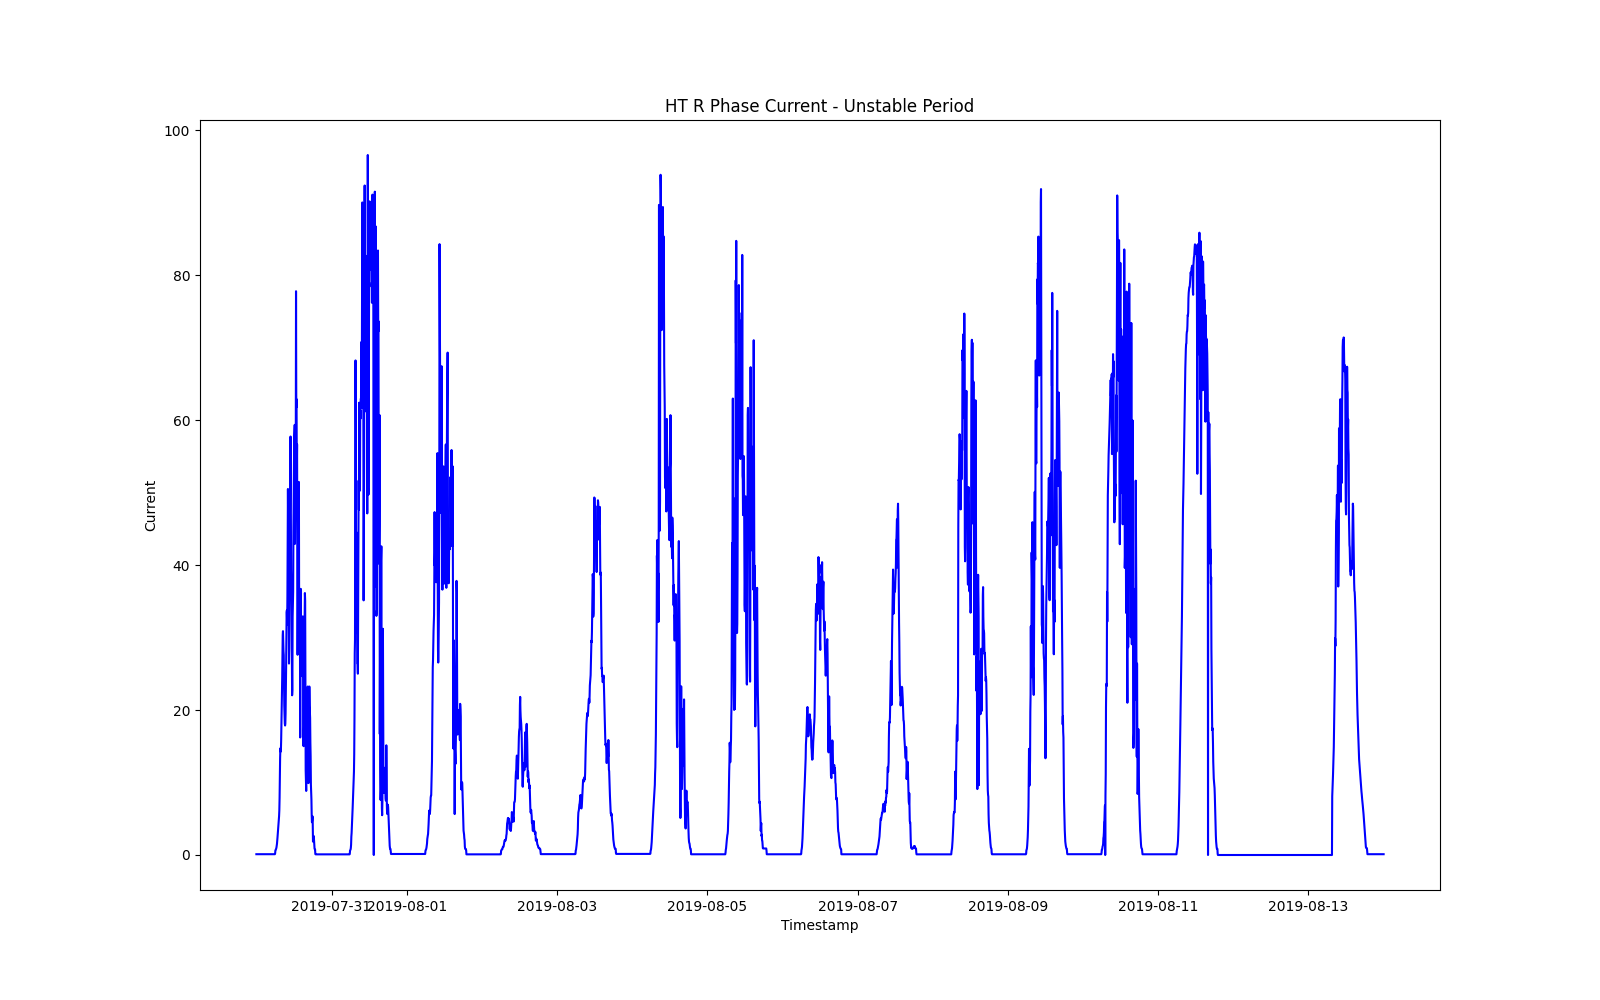
\includegraphics[width=0.65\textwidth]{./Images/unstable_period.png}
	\caption{HT R Phase Current - Unstable Period}
\end{figure}

\subsection{Removing outliers, smoothening, and imputing missing data}

Here we apply four outlier handling techniques to the unstable period: imputation, trimming, capping, and robust estimation. The results are visualized to compare the effectiveness of each method.

\begin{lstlisting}[language=Python, gobble=0]
# Method 1: Imputation (Replacing outlier values with the mean)
mean_value = unstable_period['HT R Phase Current'].mean()
median_value = unstable_period['HT R Phase Current'].median()
unstable_period['Current_Imputed_Mean'] = unstable_period['HT R Phase Current'].copy()
unstable_period.loc[(unstable_period['HT R Phase Current'] > unstable_period['HT R Phase Current'].quantile(0.95)) | (unstable_period['HT R Phase Current'] < unstable_period['HT R Phase Current'].quantile(0.05)), 'Current_Imputed_Mean'] = mean_value

unstable_period['Current_Imputed_Median'] = unstable_period['HT R Phase Current'].copy()
unstable_period.loc[(unstable_period['HT R Phase Current'] > unstable_period['HT R Phase Current'].quantile(0.95)) | (unstable_period['HT R Phase Current'] < unstable_period['HT R Phase Current'].quantile(0.05)), 'Current_Imputed_Median'] = median_value

# Method 2: Trimming (Removing outliers)
q_low = unstable_period['HT R Phase Current'].quantile(0.1)
q_high = unstable_period['HT R Phase Current'].quantile(0.9)
unstable_period_trimmed = unstable_period[(unstable_period['HT R Phase Current'] >= q_low) & (unstable_period['HT R Phase Current'] <= q_high)]

# Method 3: Capping (Setting a cap on the maximum and minimum values)
max_value = unstable_period['HT R Phase Current'].quantile(0.95)
min_value = unstable_period['HT R Phase Current'].quantile(0.05)
unstable_period['Current_Capped'] = unstable_period['HT R Phase Current'].copy()
unstable_period['Current_Capped'] = np.where(unstable_period['Current_Capped'] > max_value, max_value, unstable_period['Current_Capped'])
unstable_period['Current_Capped'] = np.where(unstable_period['Current_Capped'] < min_value, min_value, unstable_period['Current_Capped'])

# Method 4: Robust Estimation (Using RANSAC regression)
from sklearn.linear_model import RANSACRegressor, LinearRegression

# Prepare the data for RANSAC
X = unstable_period['Timestamp'].map(pd.Timestamp.timestamp).values.reshape(-1, 1)  # Convert datetime to timestamp
y = unstable_period['HT R Phase Current'].values

# Fit RANSAC
model = RANSACRegressor(LinearRegression()).fit(X, y)
unstable_period['Current_Robust'] = model.predict(X)
\end{lstlisting}

I have used the following techniques to handle the outliers:

\begin{itemize}
	\item \textbf{Imputation:} Replacing outlier values with the mean or median of the data.
	\item \textbf{Trimming:} Removing outliers from the dataset.
	\item \textbf{Capping:} Setting a cap on the maximum and minimum values.
	\item \textbf{Robust Estimation:} Using RANSAC regression to estimate the data without outliers.
\end{itemize}


\begin{figure}[H]
	\centering
	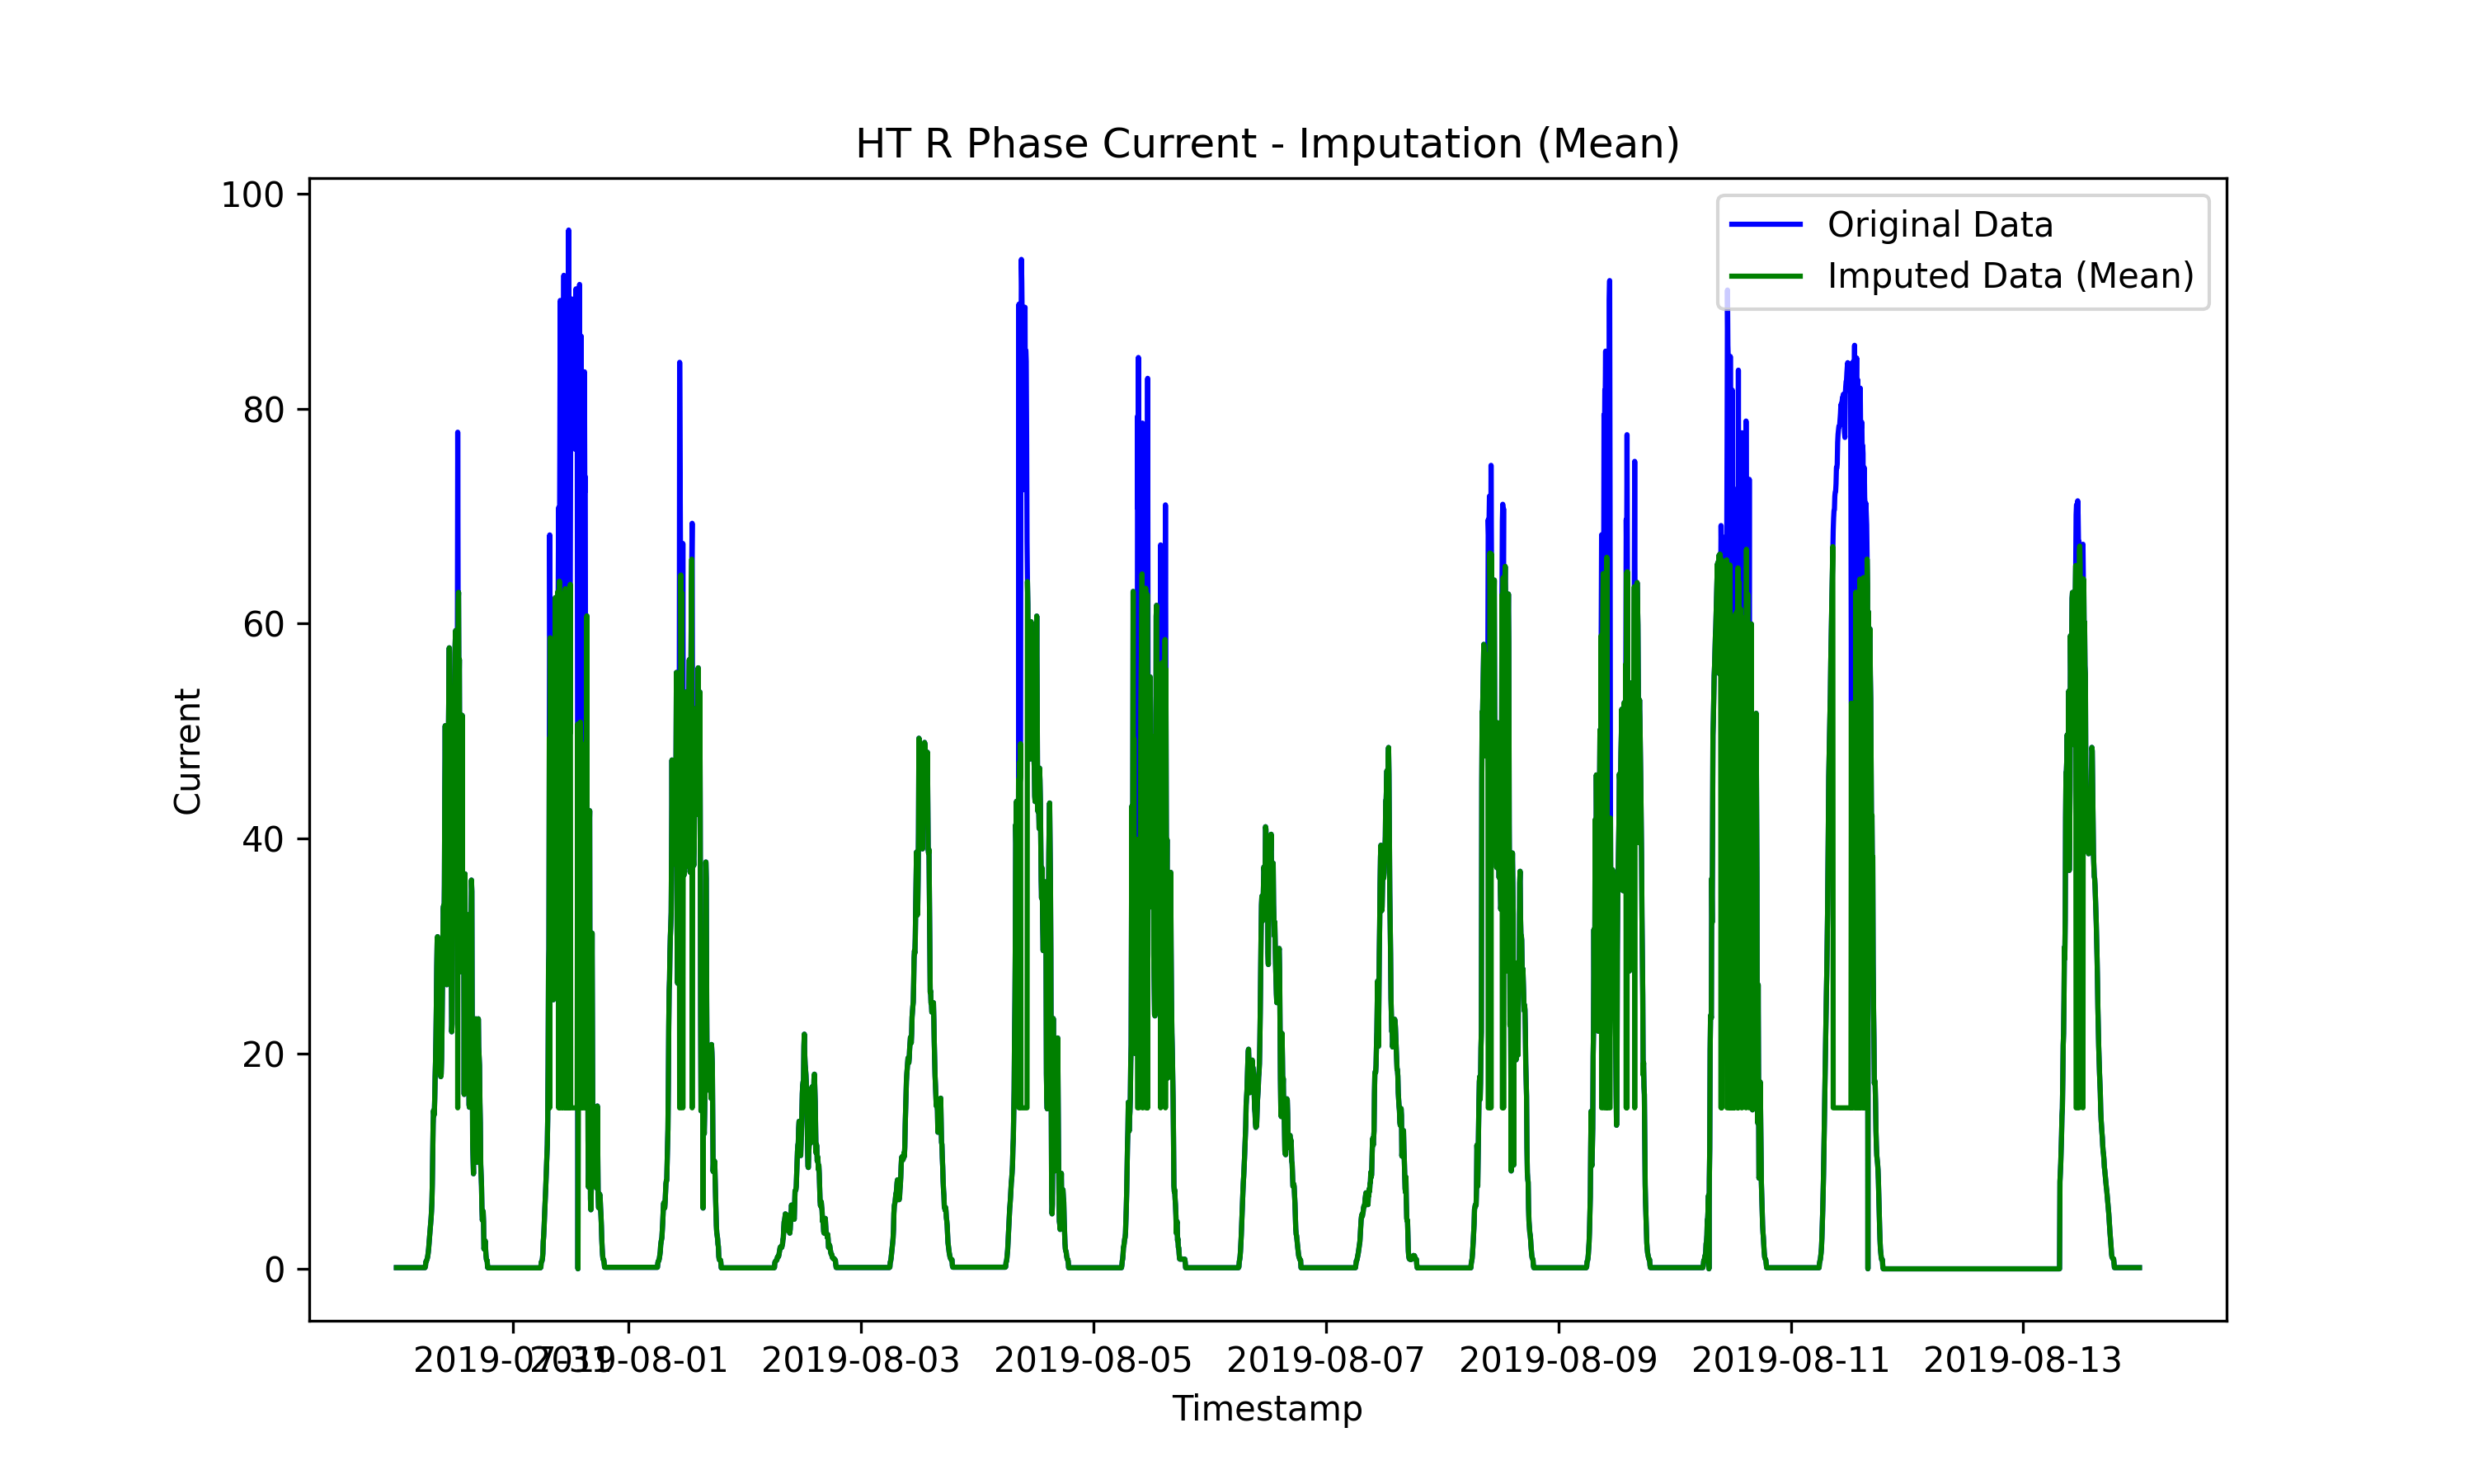
\includegraphics[width=0.9\textwidth]{./Images/imputed_mean_data.png}
	\caption{Imputed Mean Data}
\end{figure}

\begin{figure}[H]
	\centering
	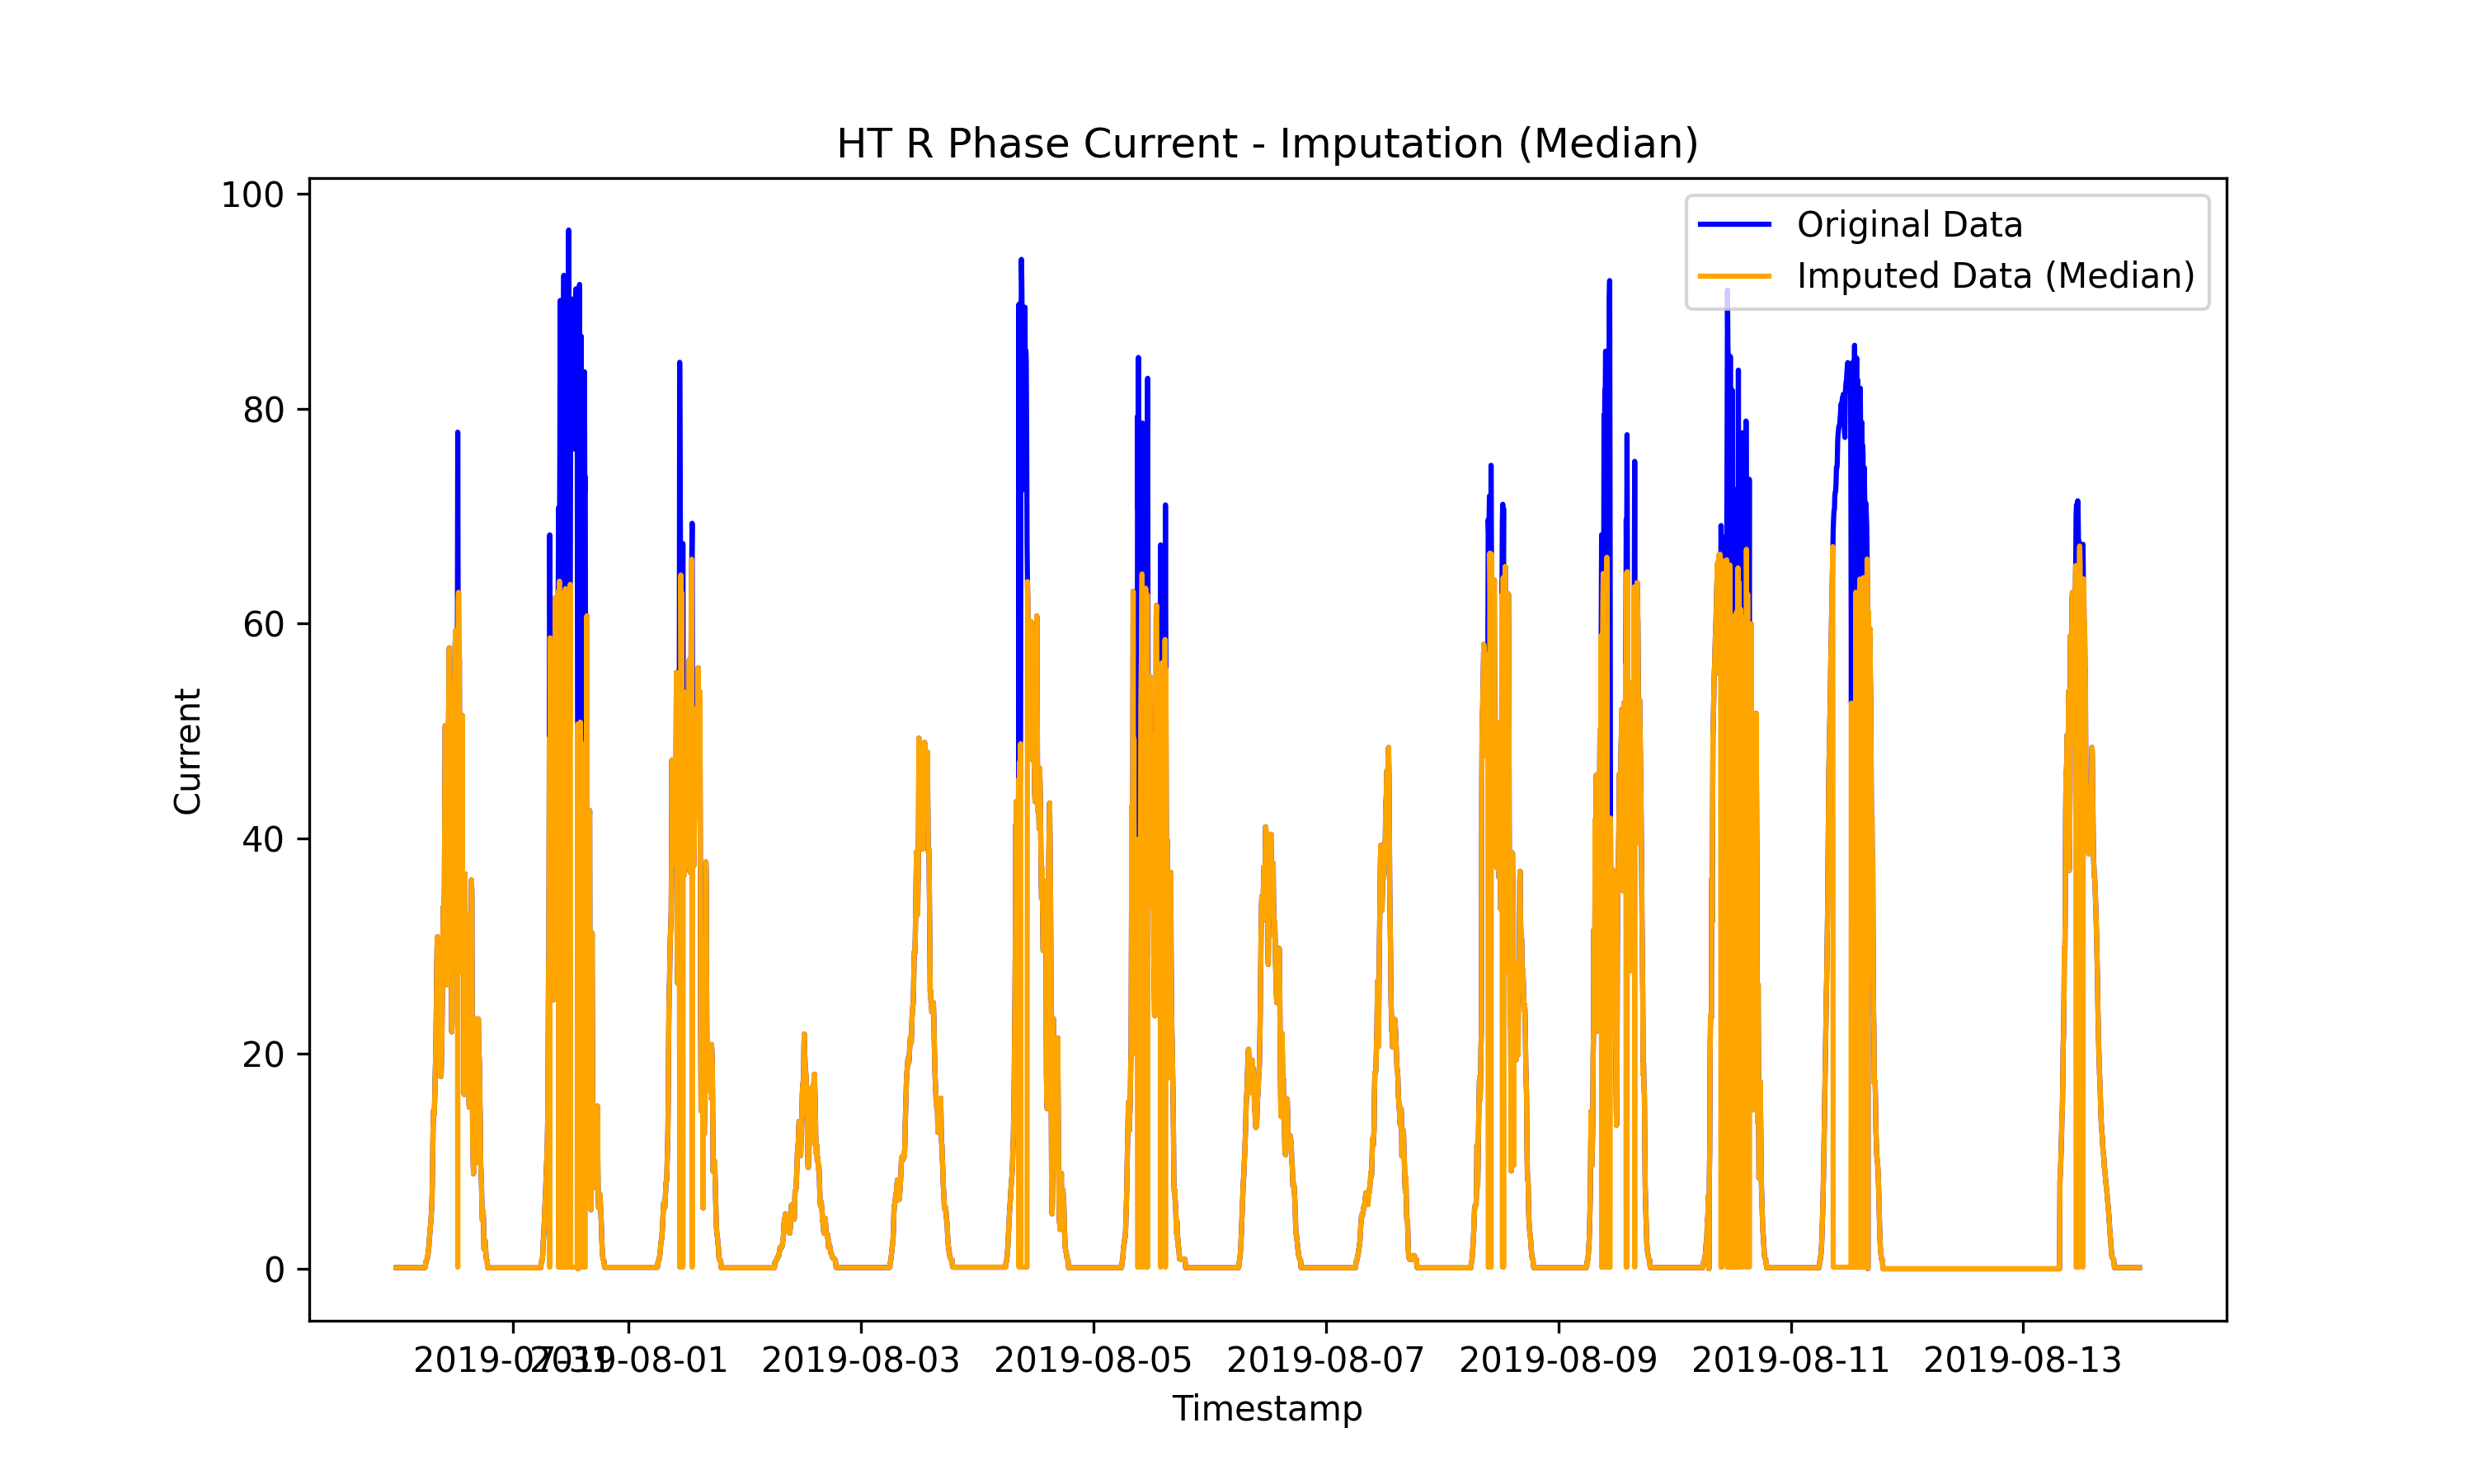
\includegraphics[width=0.9\textwidth]{./Images/imputed_median_data.png}
	\caption{Imputed Median Data}
\end{figure}

\begin{figure}[H]
	\centering
	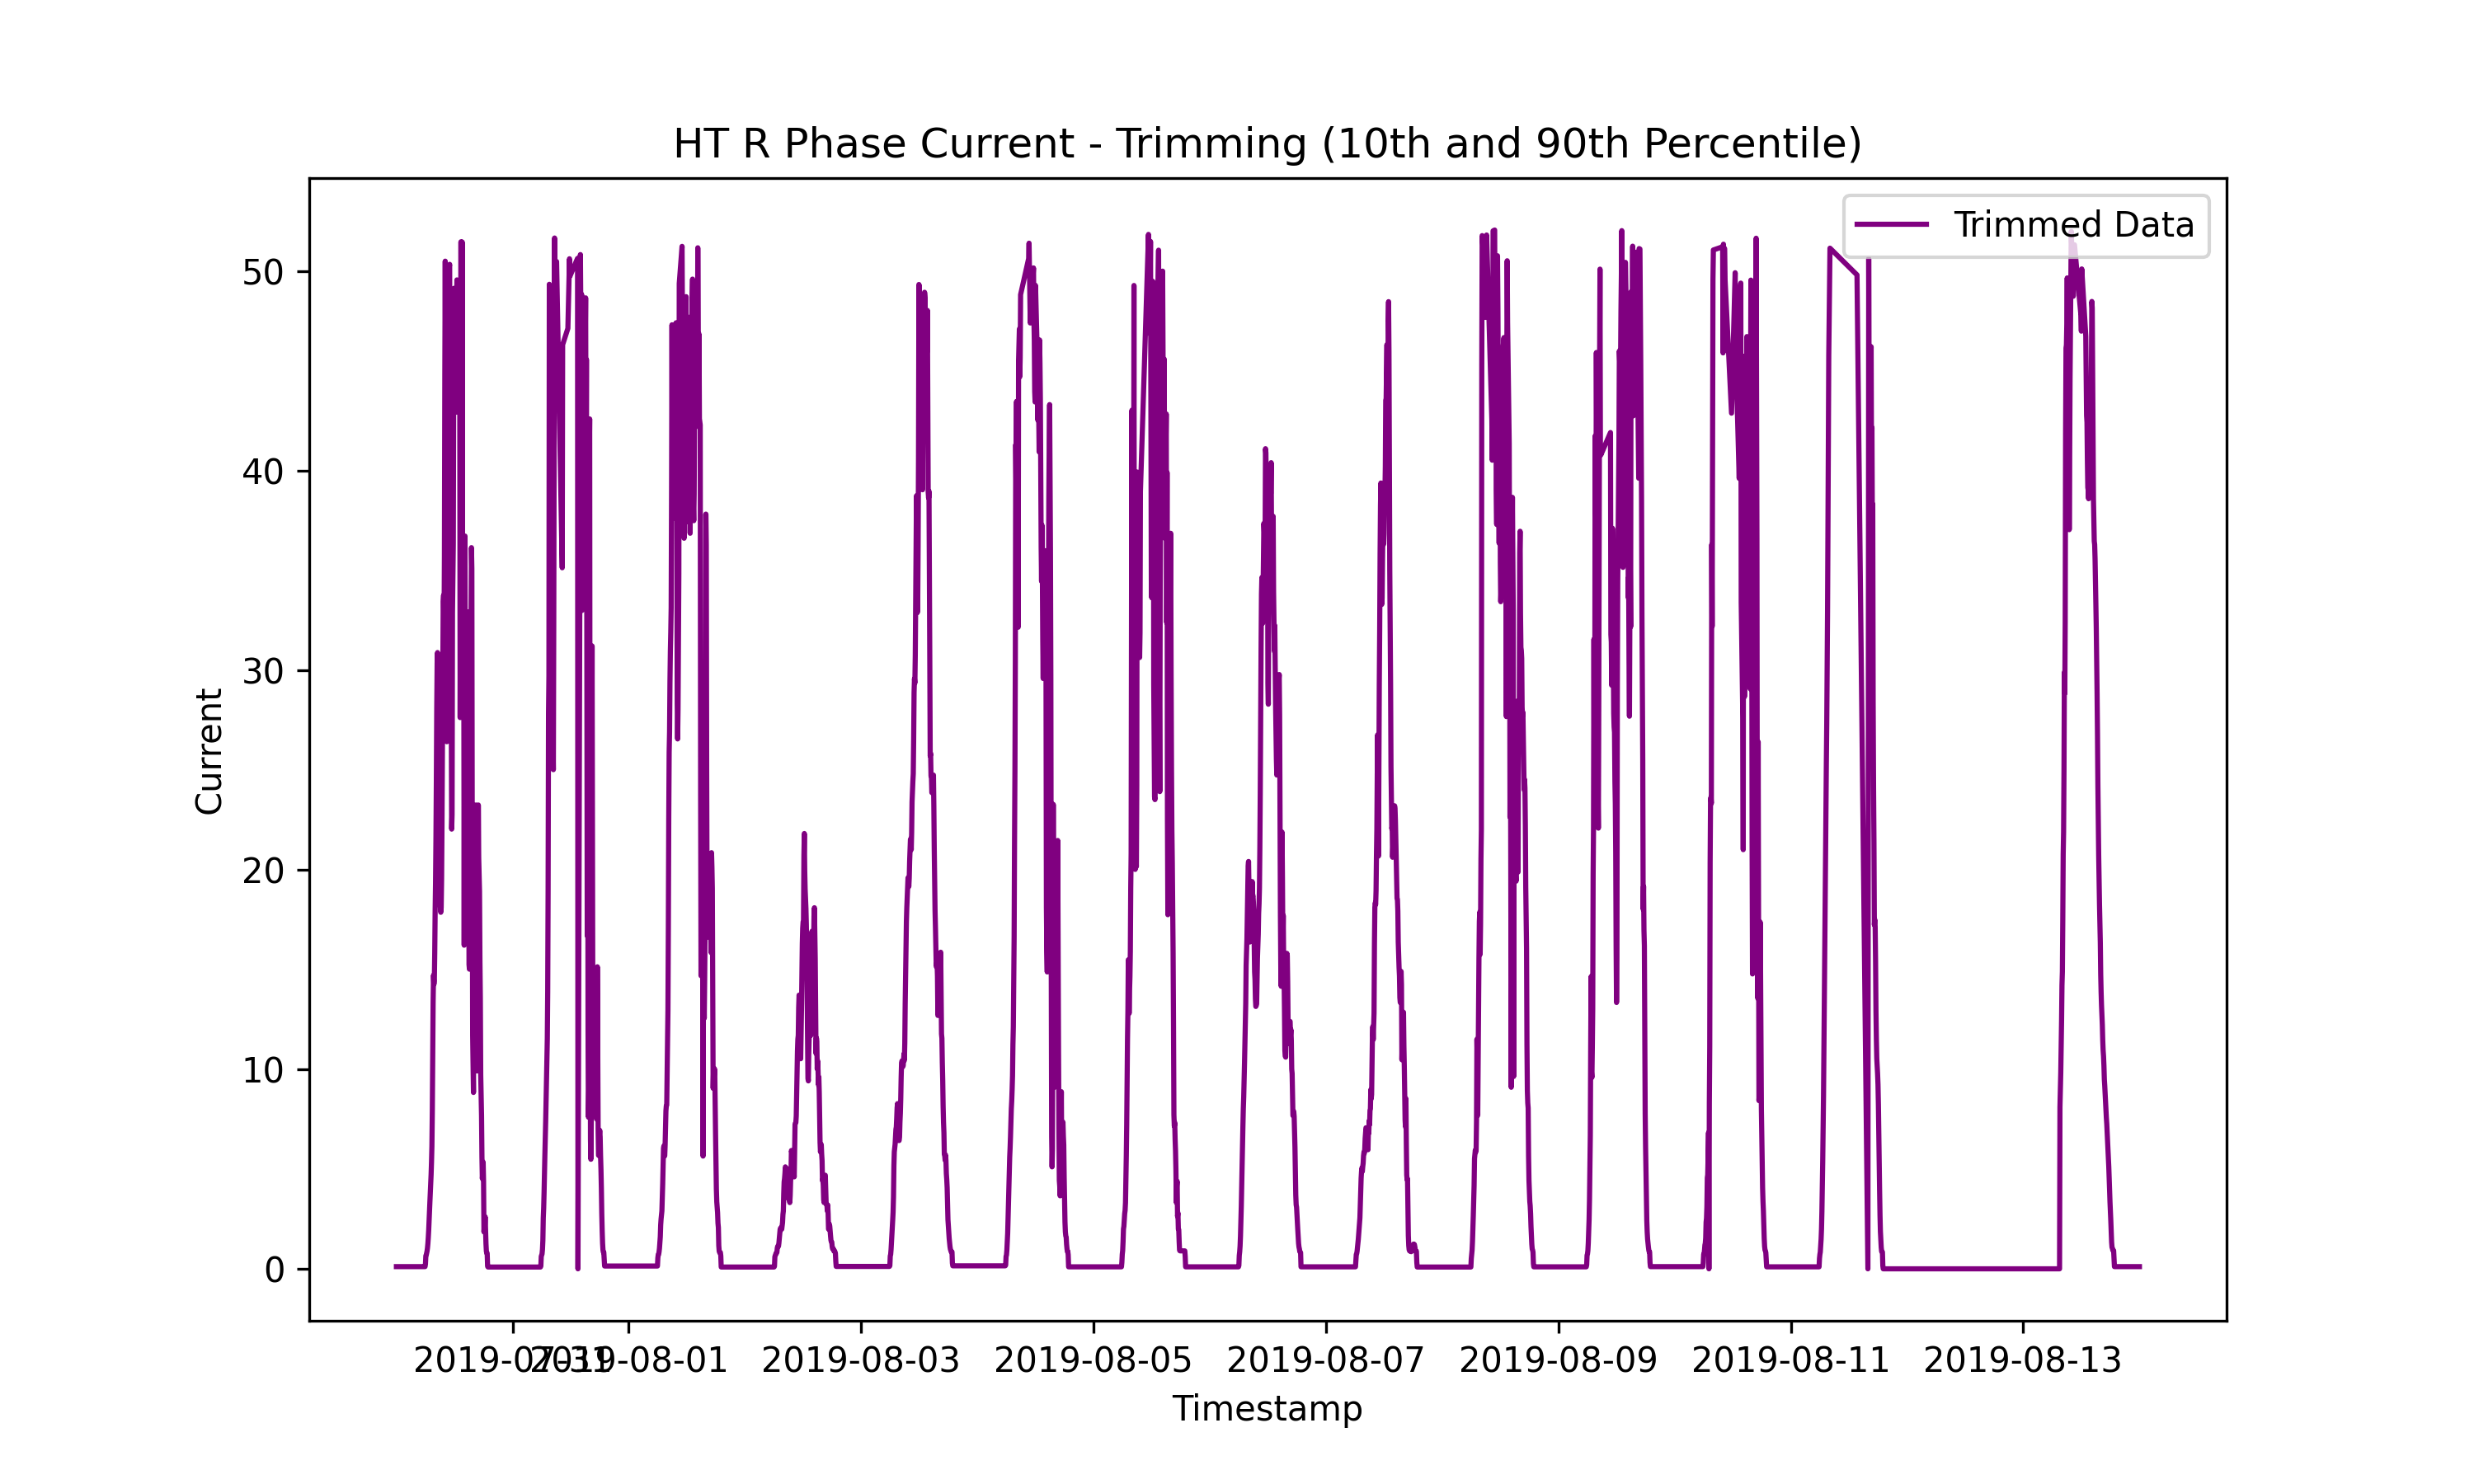
\includegraphics[width=0.9\textwidth]{./Images/trimmed_data.png}
	\caption{Trimmed Data}
\end{figure}

\begin{figure}[H]
	\centering
	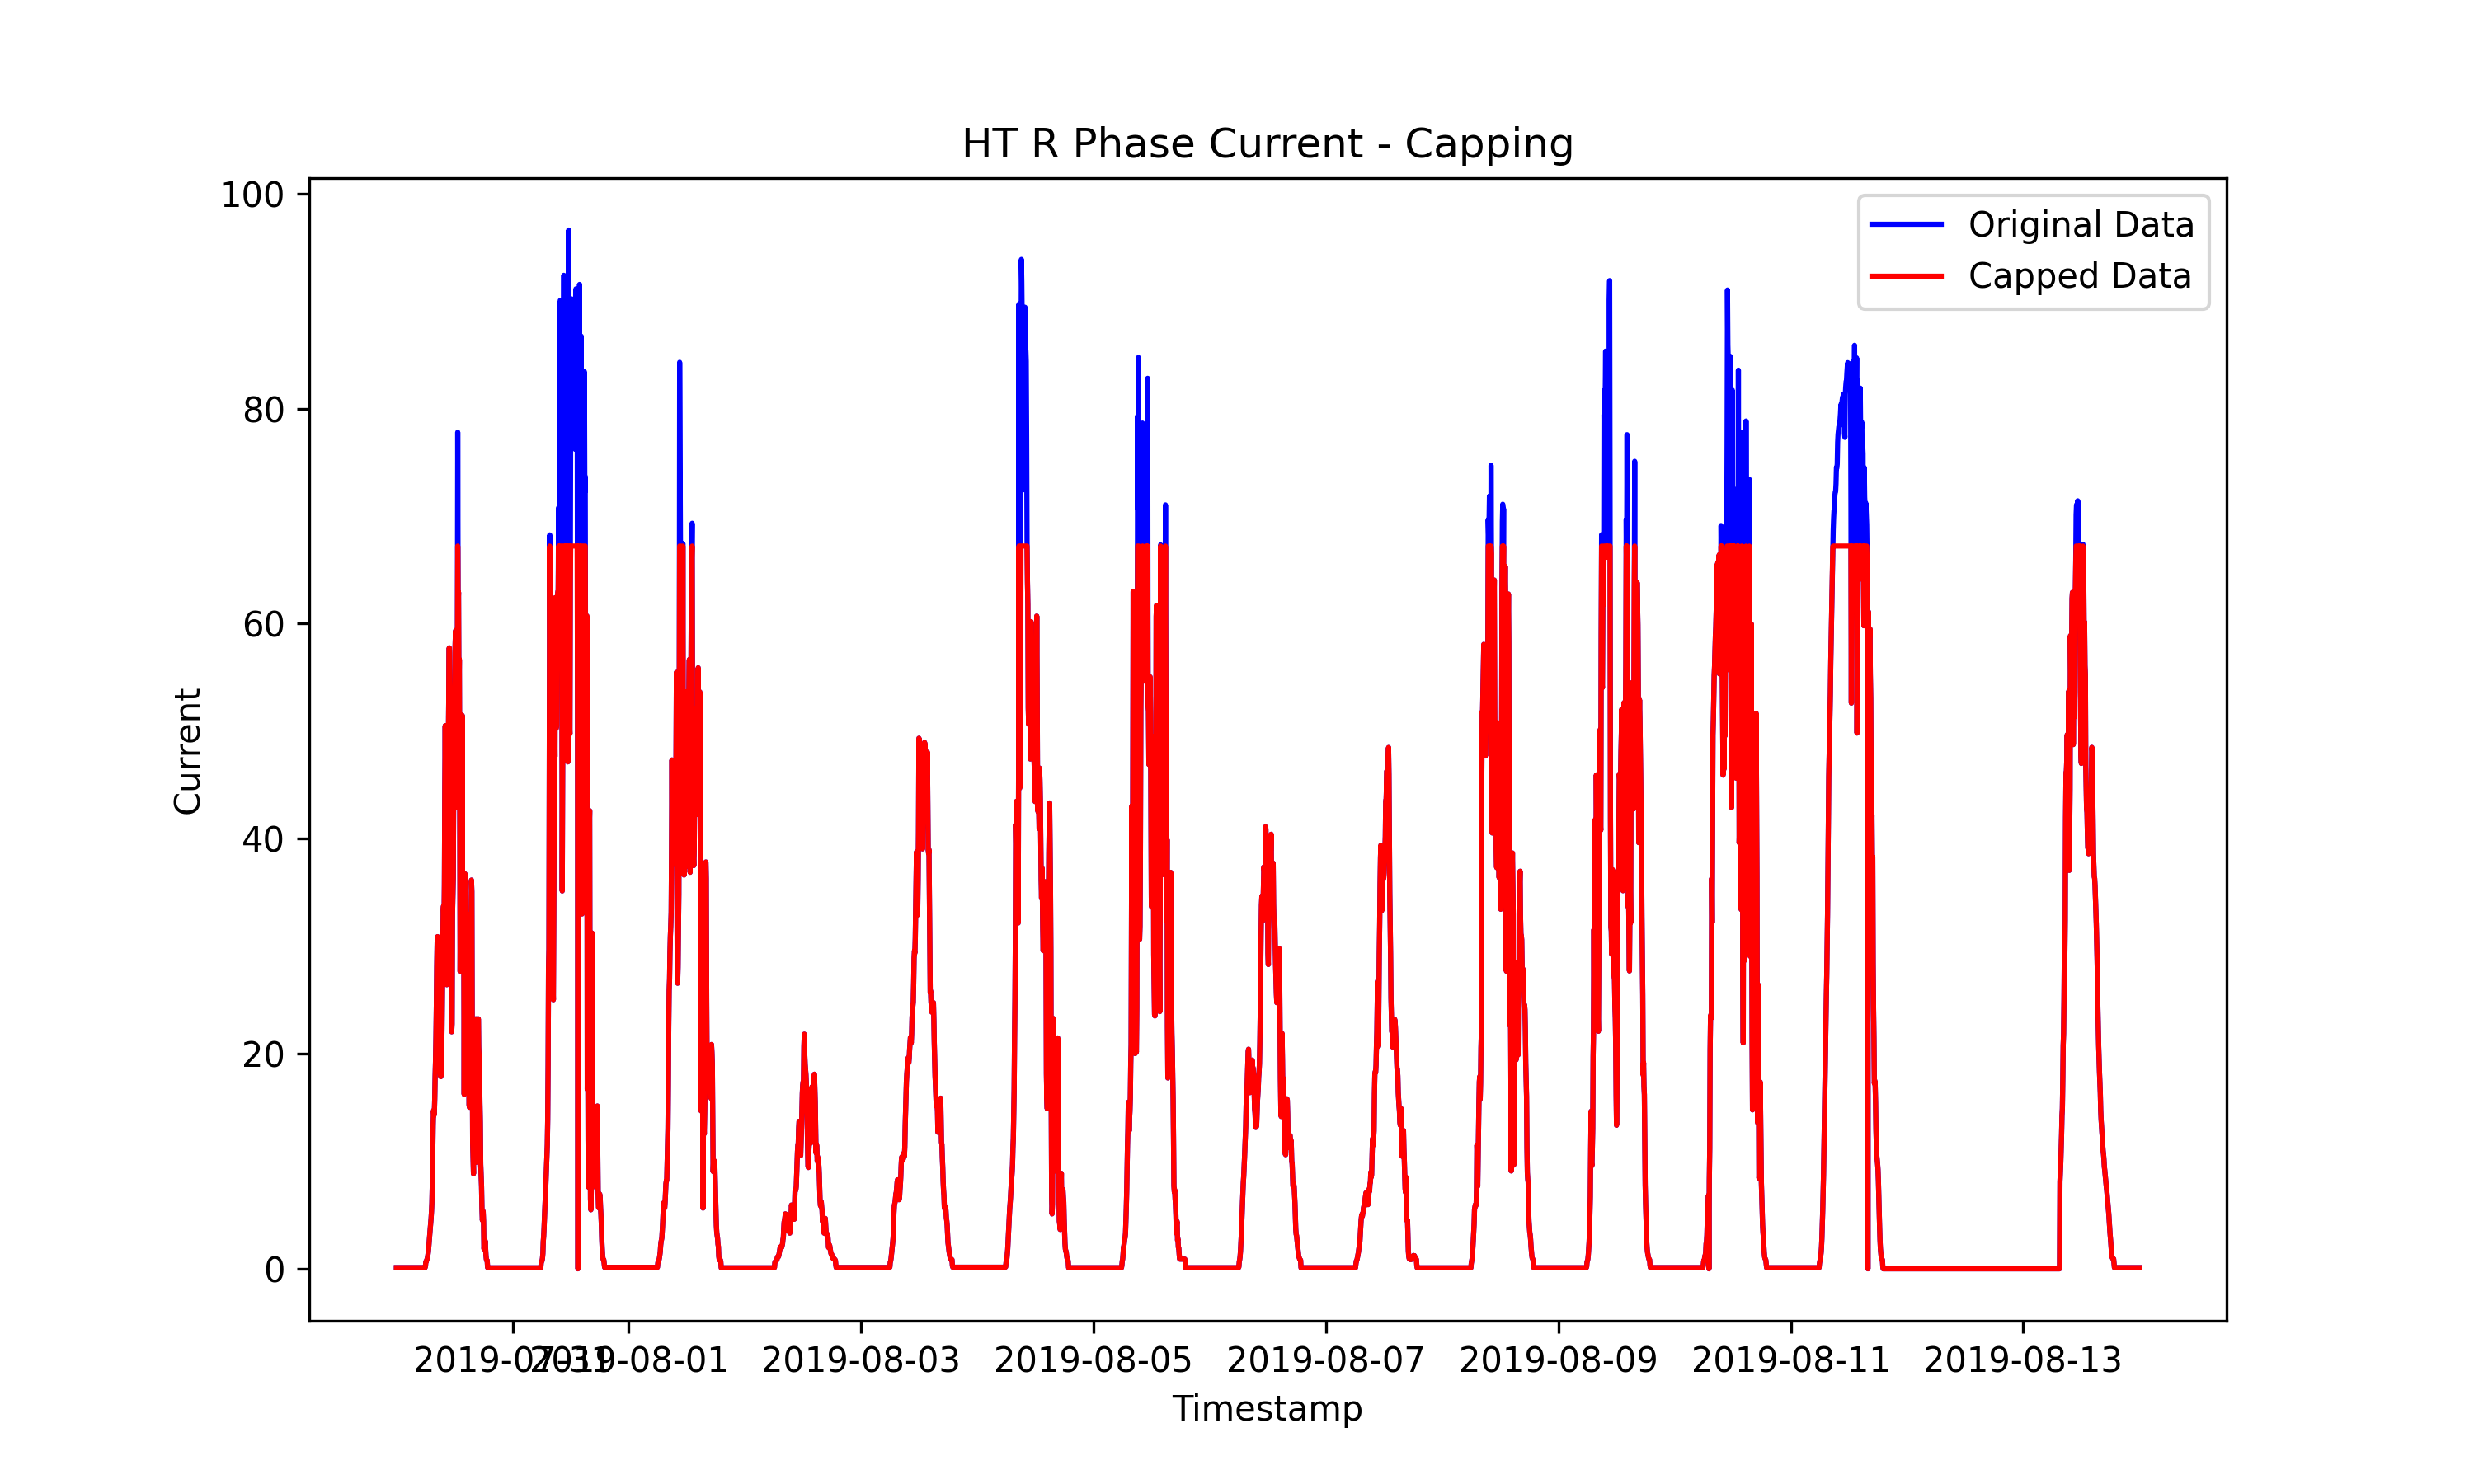
\includegraphics[width=0.9\textwidth]{./Images/capped_data.png}
	\caption{Capped Data}
\end{figure}

\begin{figure}[H]
	\centering
	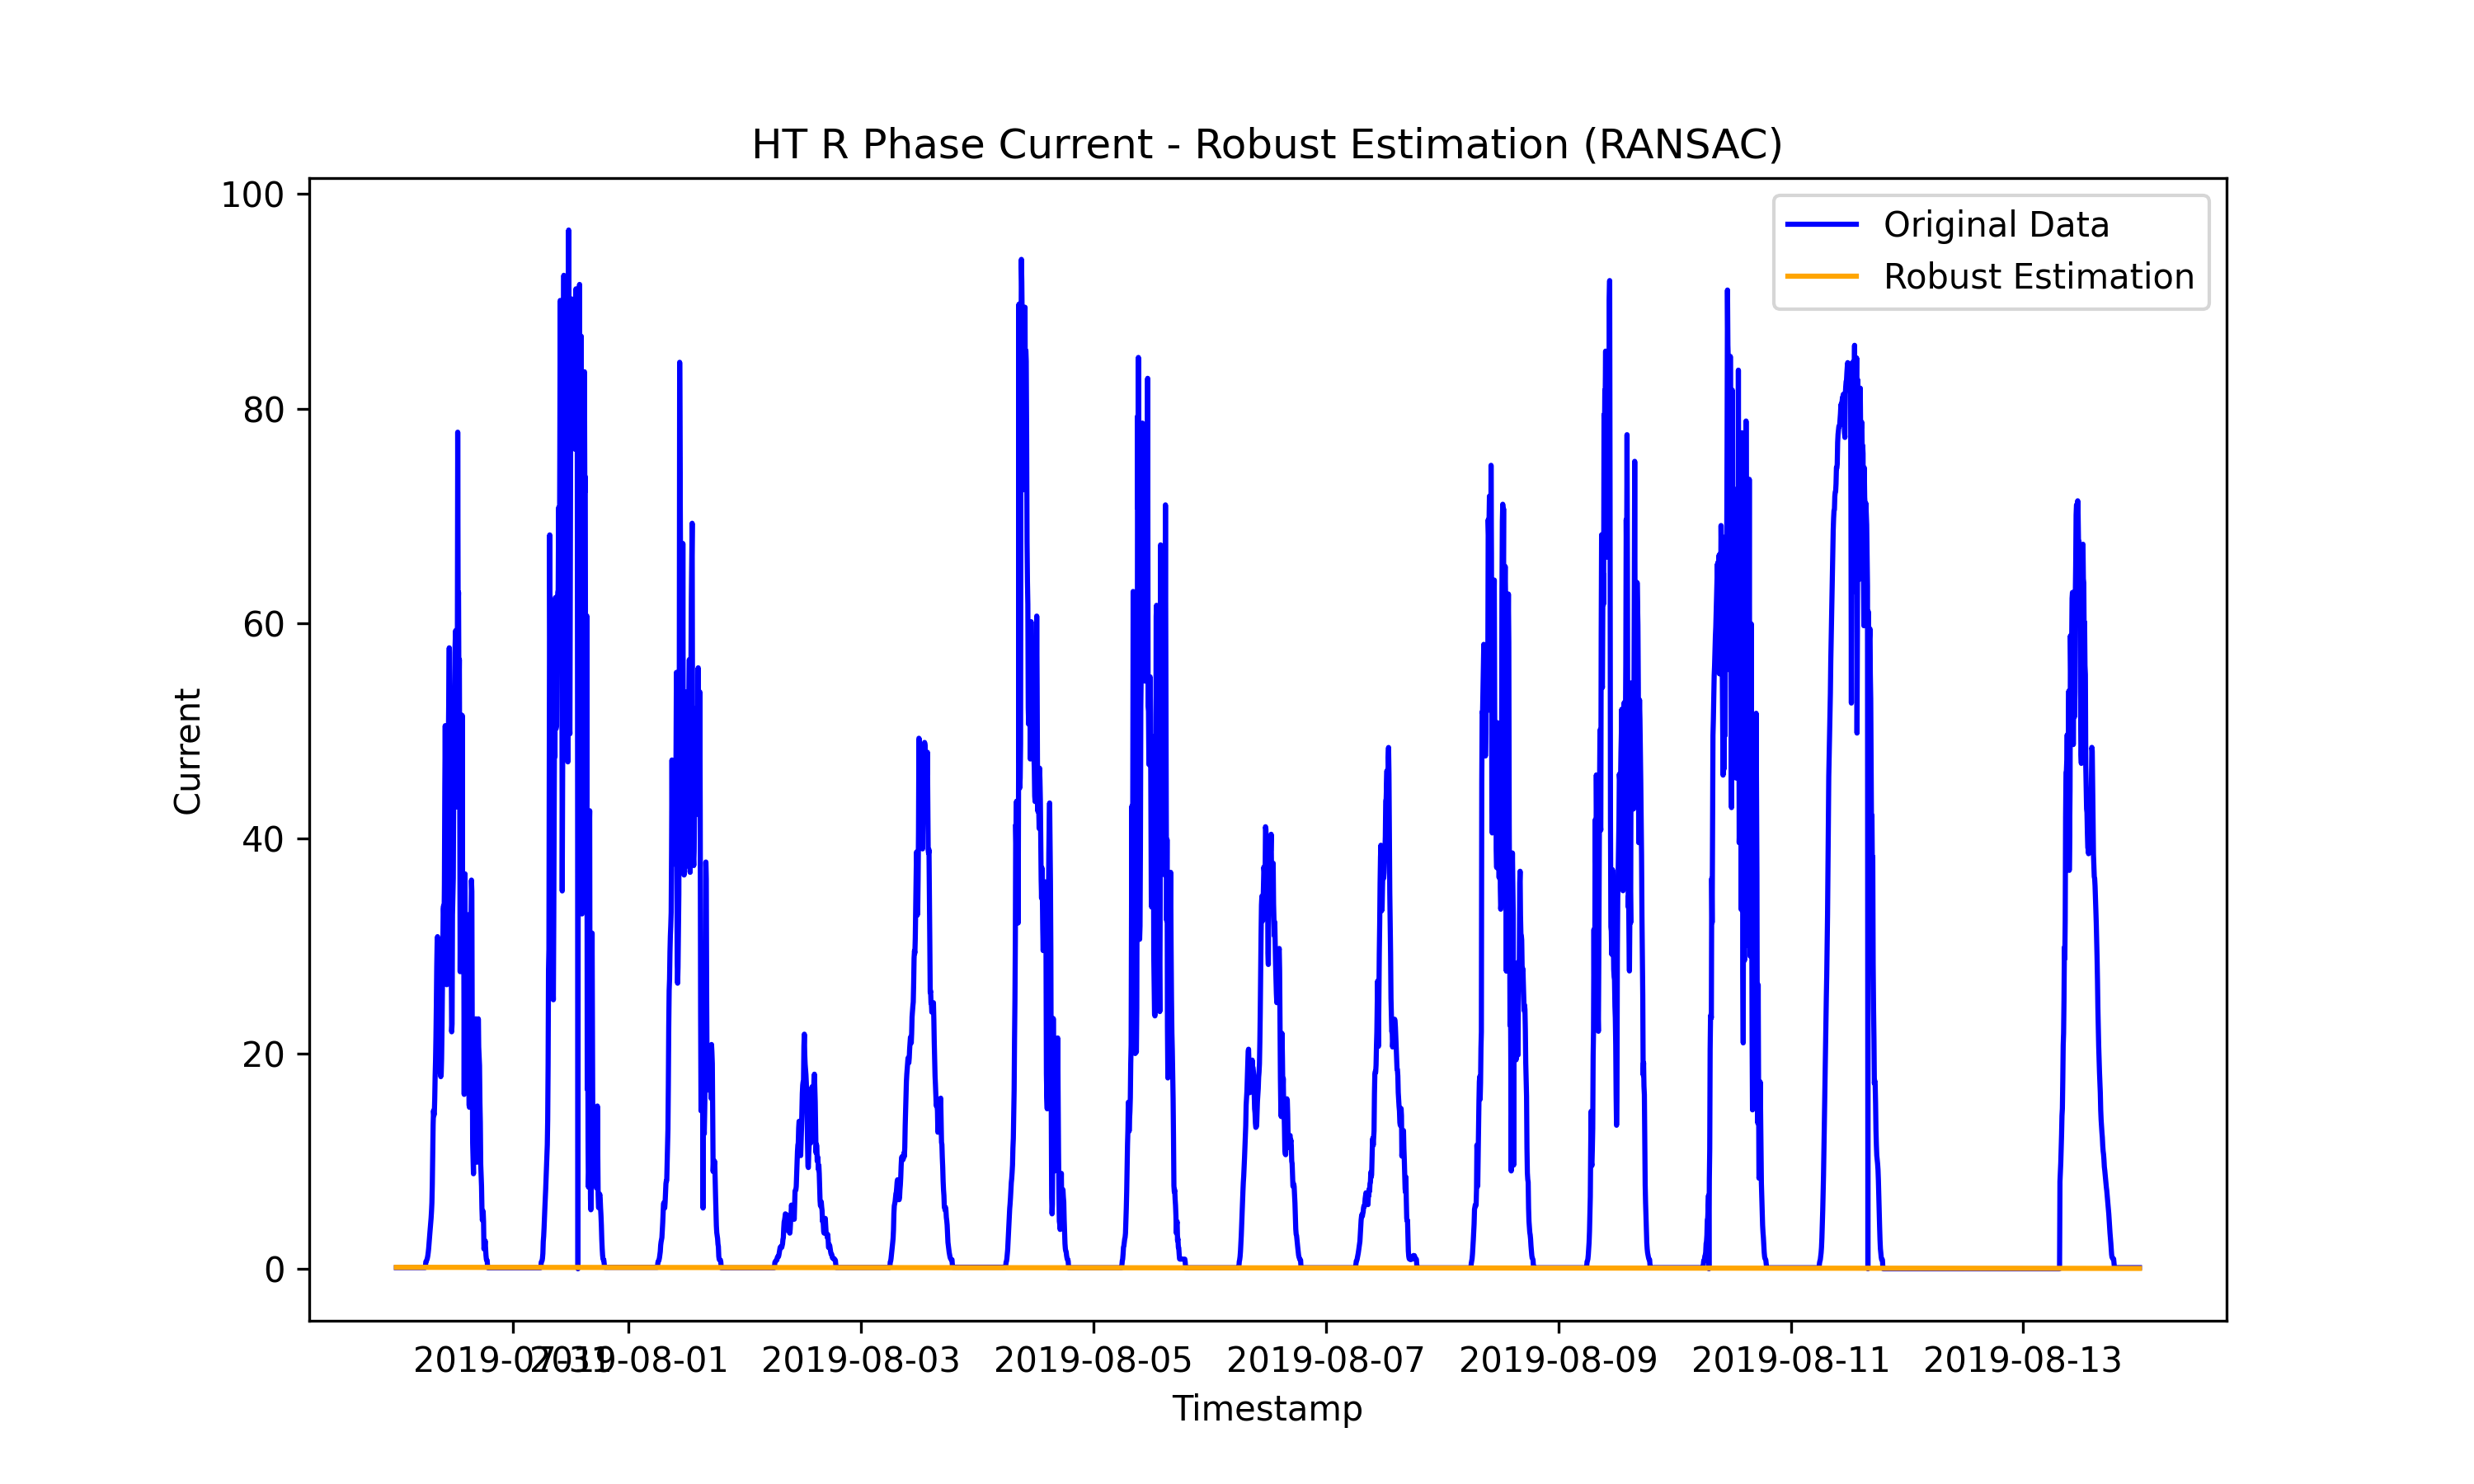
\includegraphics[width=0.9\textwidth]{./Images/robust_estimation_data.png}
	\caption{Robust Data}
\end{figure}

% Outlies Handing comparison image
\begin{figure}[H]
	\centering
	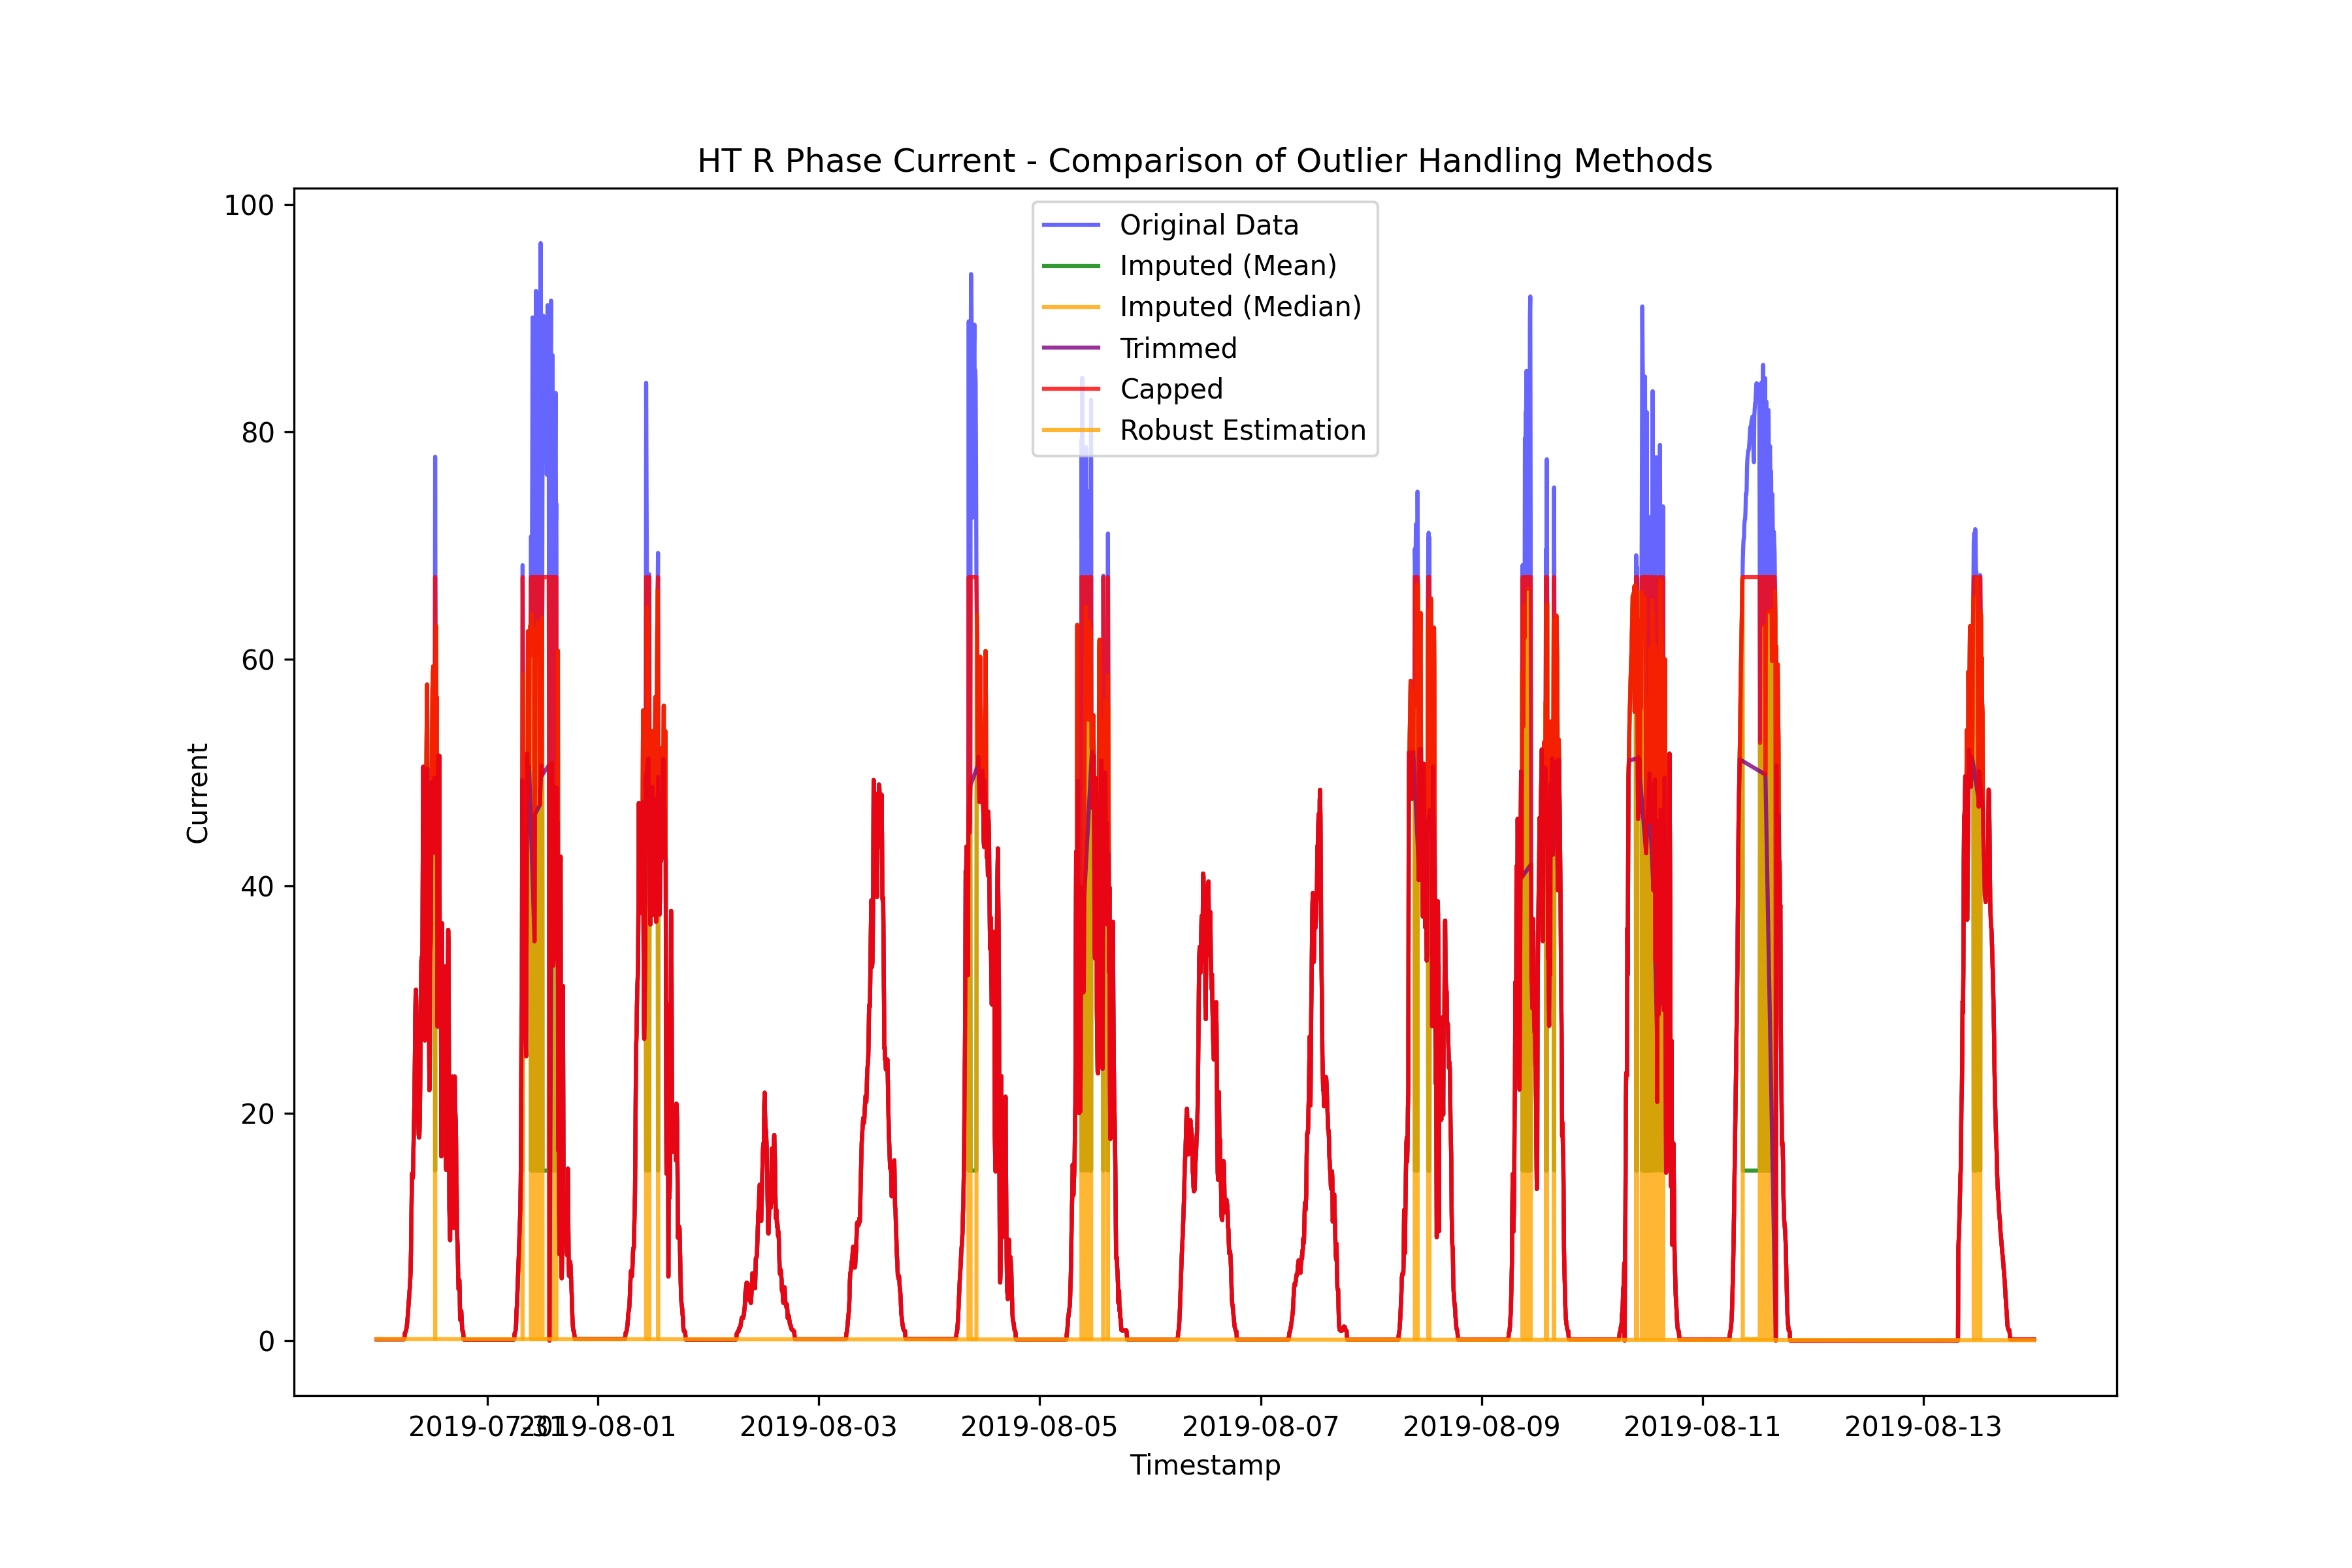
\includegraphics[width=0.9\textwidth]{./Images/outlier_handling_comparison.png}
	\caption{Outlier Handling Comparison}
\end{figure}



\clearpage